\documentclass[14pt,a4paper]{report}  %紙張設定
\usepackage{xeCJK}%中文字體模組
%\setCJKmainfont{標楷體} %設定中文字體
\setCJKmainfont{MoeStandardKai.ttf}
%\newfontfamily\sectionef{Times New Roman}%設定英文字體
\newfontfamily\sectionef{Nimbus Roman}
\usepackage{enumerate}
\usepackage{amsmath,amssymb}%數學公式、符號
\usepackage{amsfonts} %數學簍空的英文字
\usepackage{graphicx, subfigure}%圖形
\usepackage{fontawesome5} %引用icon
\usepackage{type1cm} %調整字體絕對大小
\usepackage{textpos} %設定文字絕對位置
\usepackage[top=2.5truecm,bottom=2.5truecm,
left=3truecm,right=2.5truecm]{geometry}
\usepackage{titlesec} %目錄標題設定模組
\usepackage{titletoc} %目錄內容設定模組
\usepackage{textcomp} %表格設定模組
\usepackage{multirow} %合併行
%\usepackage{multicol} %合併欄
\usepackage{CJK} %中文模組
\usepackage{CJKnumb} %中文數字模組
\usepackage{wallpaper} %浮水印
\usepackage{listings} %引用程式碼
\usepackage{hyperref} %引用url連結
\usepackage{setspace}
\usepackage{lscape}%設定橫式
\lstset{language=Python, %設定語言
		basicstyle=\fontsize{10pt}{2pt}\selectfont, %設定程式內文字體大小
		frame=lines,	%設定程式框架為線
}
%\usepackage{subcaption}%副圖標
\graphicspath{{./../images/}} %圖片預設讀取路徑
\usepackage{indentfirst} %設定開頭縮排模組
\renewcommand{\figurename}{\Large 圖.} %更改圖片標題名稱
\renewcommand{\tablename}{\Large 表.}
\renewcommand{\lstlistingname}{\Large 程式.} %設定程式標示名稱
\hoffset=-5mm %調整左右邊界
\voffset=-8mm %調整上下邊界
\setlength{\parindent}{3em}%設定首行行距縮排
\usepackage{appendix} %附錄
\usepackage{diagbox}%引用表格
\usepackage{multirow}%表格置中
%\usepackage{number line}
%=------------------更改標題內容----------------------=%
\titleformat{\chapter}[hang]{\center\sectionef\fontsize{20pt}{1pt}\bfseries}{\LARGE 第\CJKnumber{\thechapter}章}{1em}{}[]
\titleformat{\section}[hang]{\sectionef\fontsize{18pt}{2.5pt}\bfseries}{{\thesection}}{0.5em}{}[]
\titleformat{\subsection}[hang]{\sectionef\fontsize{18pt}{2.5pt}\bfseries}{{\thesubsection}}{1em}{}[]
%=------------------更改目錄內容-----------------------=%
\titlecontents{chapter}[11mm]{}{\sectionef\fontsize{18pt}{2.5pt}\bfseries\makebox[3.5em][l]
{第\CJKnumber{\thecontentslabel}章}}{}{\titlerule*[0.7pc]{.}\contentspage}
\titlecontents{section}[18mm]{}{\sectionef\LARGE\makebox[1.5em][l]
{\thecontentslabel}}{}{\titlerule*[0.7pc]{.}\contentspage}
\titlecontents{subsection}[4em]{}{\sectionef\Large\makebox[2.5em][l]{{\thecontentslabel}}}{}{\titlerule*[0.7pc]{.}\contentspage}
%=----------------------章節的間距----------------------=%
\titlespacing*{\chapter} {0pt}{0pt}{18pt}
\titlespacing*{\section} {0pt}{12pt}{6pt}
\titlespacing*{\subsection} {0pt}{6pt}{6pt}
%=----------------------標題-------------------------=%             
\begin{document} %文件
\sectionef %設定英文字體啟用
\vspace{12em}
\begin{titlepage}%開頭
\begin{center}   %標題  
\makebox[1.5\width][s] %[s] 代表 Stretch the interword space in text across the entire width
{\fontsize{24pt}{2.5pt}國立虎尾科技大學}\\[18pt]
\makebox[1.5\width][s]
{\fontsize{24pt}{2.5pt}機械設計工程系}\\[18pt]
\sectionef\fontsize{24pt}{1em}\selectfont\textbf
{
\vspace{0.5em}
cd2023 2b-pj3bg4分組報告}\\[18pt]
%設定文字盒子 [方框寬度的1.5倍寬][對其方式為文字平均分分布於方框中]\\距離下方18pt
\vspace{1em} %下移
\fontsize{30pt}{1pt}\selectfont\textbf{網際足球場景設計}\\
\vspace{1em}
\sectionef\fontsize{30pt}{1em}\selectfont\textbf
{
\vspace{0.5em}
Web-based Football Scene Design}
 \vspace{2em}
%=---------------------參與人員-----------------------=%             
\end{center}
\begin{flushleft}
\begin{LARGE}

\hspace{32mm}\makebox[5cm][s]
{指導教授:\quad 嚴\quad 家\quad 銘\quad 老\quad 師}\\[6pt]
\hspace{32mm}\makebox[5cm][s]
{班\qquad 級:\quad 四\quad 設\quad 二\quad 乙}\\[6pt]
\hspace{32mm}\makebox[5cm][s]
{學\qquad 生:\quad 陳\quad 冠\quad 佑\quad(41023219)}
\\[6pt]
\hspace{32mm}\makebox[5cm][s]
{\hspace{36.5mm}陳\quad 冠\quad 翰\quad(41023221)}\\[6pt]
\hspace{32mm}\makebox[5cm][s]
{\hspace{36.5mm}陳\quad 奕\quad 倫\quad(41023222)}\\[6pt]
\hspace{32mm}\makebox[5cm][s]
{\hspace{36.5mm}陳\quad 王晉\quad 維\quad(41023228)}\\[6pt]
\hspace{32mm}\makebox[5cm][s]
{\hspace{36.5mm}黃\quad 仕\quad 鈞\quad(41023234)}\\[6pt]
\hspace{32mm}\makebox[5cm][s]
{\hspace{36.5mm}劉\quad 學\quad 宇\quad(41023247)}\\[6pt]
\hspace{32mm}\makebox[5cm][s]
{\hspace{36.5mm}鄭\quad 立\quad 揚\quad(41023251)}\\[6pt]
\hspace{32mm}\makebox[5cm][s]
{\hspace{36.5mm}謝\quad 鴻\quad 元\quad(41023254)}\\[6pt]
\hspace{32mm}\makebox[5cm][s]

%設定文字盒子[寬度為5cm][對其方式為文字平均分分布於方框中]空白距離{36.5mm}\空白1em
\end{LARGE}
\end{flushleft}
\vspace{6em}
\fontsize{18pt}{2pt}\selectfont\centerline{\makebox[\width][s]
{中華民國\hspace{3em} 
112 \quad 年\quad 5\quad 月}}
\end{titlepage}
\newpage
%=---------------報告製作核可證明---------------------=%
 {\renewcommand\baselinestretch{1.4}\selectfont %設定以下行距
 {\begin{center}
    {\fontsize{20pt}{2.5pt} {國立虎尾科技大學 \qquad 機械設計工程系}\\[8pt]{分組報告製作合格認可證明}\\
    \hspace*{\fill} \\ %似enter鍵換行
    \par}
     \end{center}}
    {\begin{textblock}{60}(1.85,0.8)
    \noindent \fontsize{15pt}{16pt}\selectfont 分組報告製作修習學生\enspace:\quad
    {\begin{minipage}[t]{10em}\underline{四設二乙\enspace 41023219 陳冠佑}\\\underline{四設二乙\enspace 41023221 陳冠翰}\\\underline{四設二乙\enspace 41023222 陳奕倫}\\\underline{四設二乙\enspace 41023228 陳瑨維}\\\underline{四設二乙\enspace 41023234 黃仕鈞}\\ \underline{四設二乙\enspace 41023247\enspace 劉學宇}\\ \underline{四設二乙\enspace 41023251\enspace 鄭立揚}\\ \underline{四設二乙\enspace 41023254\enspace 謝鴻元}\\ %下劃線符號指令
    \end{minipage}}
         \par} %結束指定行距
    {\renewcommand\baselinestretch{1.2}\selectfont %設定以下行距
    {\begin{textblock}{30}(1.8,4)
    \noindent \fontsize{16pt}{16pt}\selectfont 分組報告題目\enspace :網際足球場景設計
    \hspace*{\fill} \\
    \hspace*{\fill} \\
    \noindent \fontsize{16pt}{16pt}\selectfont 經評量合格,特此證明
    \hspace*{\fill} \\
    \hspace*{\fill} \\
    \noindent \fontsize{16pt}{16pt} \makebox[6em][s]{評審委員}\enspace:\quad
    {\begin{minipage}[t]{6em} \underline{            }\\[16pt] \underline{            }\\[16pt] \underline{            }\\
    \end{minipage}}
    \end{textblock}}
    {\begin{textblock}{10}(1.8,9)
    {\begin{flushleft}
    \fontsize{16pt}{16pt}\selectfont \makebox[6em][s]{指導老師}\enspace:\quad \underline{            }\\[10pt]
    \hspace*{\fill} \\
    \fontsize{16pt}{2.5pt}\selectfont \makebox[12em][s]{中華民國一一二年}\hspace{2pt}
    \fontsize{16pt}{2.5pt}\selectfont\makebox[8em][s]{五月十二日}
    \end{flushleft}}
    \end{textblock}}
    \end{textblock}}
     \par} %結束指定行距
     \newpage

%=------------------------摘要-----------------------=%
\renewcommand{\baselinestretch}{1.5} %設定行距
\pagenumbering{roman} %設定頁數為羅馬數字
\clearpage  %設定頁數開始編譯
\sectionef
\addcontentsline{toc}{chapter}{摘~~~要} %將摘要加入目錄

\begin{center}
\LARGE\textbf{摘~~要}\\
\end{center}

\begin{flushleft}

\fontsize{14pt}{20pt}\sectionef\hspace{12pt}\quad 此專題是運用bubblerob,將其導入 CoppeliaSim 模擬環境並給予對應設置,將其程式系統化並運用 zmq Remote api進行控制,找到適合此場景的程式寫法後,再到 CoppeliaSim 模擬環境中進行測試程式和場景在多人連線中的可行性。並嘗試透過架設伺服器將 CoppeliaSim 影像串流到網頁供使用者觀看或操控。


\end{flushleft}

\begin{center}
\fontsize{14pt}{20pt}\selectfont 關鍵字: 影像串流\sectionef bubblerob、zmq Remote api、CoppeliaSim
\end{center}

\newpage
\renewcommand{\baselinestretch}{1.5} %設定行距

%=------------------------誌謝----------------------=%
\begin{center}	
\addcontentsline{toc}{chapter}{誌~~~謝}
\LARGE\textbf{誌~~謝}\\
\end{center}
\begin{center}
\begin{flushleft}
\fontsize{14pt}{20pt}\sectionef\hspace{12pt}\quad 在此鄭重感謝製作以及協助本分組報告完成的所有人員,首先向嚴家銘老師致謝,他們不辭辛勞解決我們的提問,甚至從來沒有不耐煩,總是貼心為我們找出最佳解答。再來是其他組的同學,提供我們解決問題的建議,最後是由本分組成員同心協力才得以完成本報告,特此感謝。
\end{flushleft}
\newpage
%=------------------------目錄----------------------=%
\renewcommand{\contentsname}{\centerline{\fontsize{18pt}{\baselineskip}\selectfont\textbf{目\quad 錄}}}
\tableofcontents  %目錄產生
\newpage
%=------------------圖表目錄產生----------------------=%
\renewcommand{\listfigurename}{\centerline{\fontsize{18pt}{\baselineskip}\selectfont\textbf{圖\quad 目\quad 錄 }}}
\newcommand{\loflabel}{圖} %定義\loflabel 文字為圖
\renewcommand{\numberline}[1]{\loflabel~#1\hspace*{0.5em}}
\listoffigures
%\newcommand{\captioname}{圖}
\newpage
\renewcommand{\listtablename}{\centerline{\fontsize{18pt}{\baselineskip}\selectfont\textbf{表\quad 目\quad 錄 }}}
\newcommand{\lotlabel}{表} %定義\lotlabel 文字為表
\renewcommand{\numberline}[1]{\lotlabel~#1\hspace*{0.5em}}
\listoftables

\end{center}
%=-------------------------內容----------------------=%

\chapter{更新網站步驟}
\section{詳細步驟說明}


 1.個人的fork倉儲點選sync fork\\

2.輸入git pull\\

3.進行編輯\\

4.acp\\

5.從個人fork 倉儲Open pull request\\

6.回到整組倉儲merge pull request\\


\chapter{Instruction}
\section{Cmd}

dir (查看目錄)\\

help (指令求救)\\

python +名(利用python執行"+名"檔案)\\

cls (清除指令紀錄)\\

cd +名 (移動)\\

檔名開頭+TAB鍵 (列出全名-可連續按)\\

attrib -r -s -h X:\. /s /d (將X槽的檔案從隱藏還原)\\

\section{Git}


git add (存取資料)\\

git commit -m "name" (命名此批欲上傳資料)\\

git pull (更新至近端資料)\\

git push (上傳至遠端)\\

git version (查看git版本)\\

git update (更新github版本)\\

git revert -m "name"(還原commit -m name紀錄)\\

git cleav -n -f(-n列出欲清除的資料 -f真的清除)\\

git status (狀態查詢)\\

git branch +名 (新建分支)\\

git checkout +名 (切換分支)\\

git merge +名 (合併分支)\\

git log (查看檔案版本)\\

git log --oneline --graph --all (檢查各版本間的關聯與樹狀圖)\\


\chapter{group}

\section{列出所有成員資料}
\begin{lstlisting}[language=Python, frame=single, numbers=left, captionpos=b, basicstyle=\ttfamily\small, showstringspaces=false, breaklines=true, tabsize=4, xleftmargin=15pt]
from browser import html, document
brython_div = document["brython_div1"]
# 在預警退選結束後, 已經不需要從教務主機讀取學員選課資料, 可以直接從 studlist 取得
stud_data = "https://mde.tw/studlist/2023spring/2b.txt"
# 先確定可以取得各欄位的資料
# 利用 open() 開啟網站連結, 之後透過 readlines() 將每一行放入 list
data = open(stud_data).readlines()
# 查驗是否完整讀取所有學員資料
#print(len(data[1:]))
# 接著以 for 迴圈逐一讀出數列時, 同時去除最後的 \print
# resume 倉儲與網站連結樣板
repo = "https://github.com/mdecd2023/"
site = "https://mdecd2023.github.io/"
resume_repo = repo + "resume-"
resume_site = site + "resume-"
football_repoa = repo + "football-apj1"
football_repob = repo + "football-bpj1"
football_sitea = site + "football-apj1"
football_siteb = site + "football-bpj1"
pj1_repoa = repo + "2a-"
pj1_repob = repo + "2b-"

pj1_sitea = site + "2a-"
pj1_siteb = site + "2b-"

pj2_repoa = repo + "2a2-"
pj2_repob = repo + "2b2-"

pj2_sitea = site + "2a2-"
pj2_siteb = site + "2b2-"

pj3_repoa = repo + "2a3-"
pj3_repob = repo + "2b3-"

pj3_sitea = site + "2a3-"
pj3_siteb = site + "2b3-"

for i in data[1:]:
    # 因為 data 第一列為資料標題, 可以利用 data[1:] 去除
    # 而數列中每一個 element 最後的跳行符號 \n 可以利用 strip() 去除
    stud_list = i.strip().split("\t")
    stud_num = stud_list[0]
    try:
        # 若無 github 帳號則設為學號
        github = stud_list[1]
    except:
        github = stud_num
    try:
        pj1 = stud_list[2]
    except:
        pj1 = "pj0"
    try:
        pj2 = stud_list[3]
    except:
        pj2 = "pj0"
    try:
        pj3 = stud_list[4]
    except:
        pj3 = "pj0"
    #print(stud_num, github, pj1, pj2, pj3)
    # 各學員 resume 倉儲連結
    resume = html.A("resume", href=resume_repo+str(github))
    football = html.A("football", href=football_siteb)
    football_repo = html.A("repo", href=football_repob)
    pj1_site = html.A("pj1", href=pj1_siteb+pj1)
    pj1_repo = html.A("repo", href=pj1_repob+pj1)
    pj2_site = html.A("pj2", href=pj2_siteb+pj2)
    pj2_repo = html.A("repo", href=pj2_repob+pj2)
    pj3_site = html.A("pj3", href=pj3_siteb+pj3)
    pj3_repo = html.A("repo", href=pj3_repob+pj3)
    brython_div <= stud_num+": "+resume+", "+football+" ("+\
                   football_repo+"), "+pj1_site+" ("+pj1_repo+")"+\
                   ", "+pj2_site+" ("+pj2_repo+")"+\
                   ", "+pj3_site+" ("+pj3_repo+")"
 
    brython_div <= html.BR()
print("done")
'''
acd_tem = "https://mdecd2023.github.io/2a2-pj2ag"
agithub = "https://github.com/mdecd2023/2a2-pj2ag"
brython_div = document["brython_div1"]
for i in range(1, 12):
    url = acd_tem + str(i)
    github = agithub + str(i)
    brython_div <= html.A("pj2ag"+str(i), href=url)
    brython_div <= " ("
    brython_div <= html.A("repo", href=github)
    brython_div <= ")"
    brython_div <= html.BR()
'''\end{lstlisting}
\chapter{會議記錄}


\section{5/24會議紀錄}


討論事項:分配工作、討論機器人規格\\


工作分配:\\
畫圖:41023234、41023247\\
PDF:41023228、41023251\\
程式:41023228、41023251、41023254\\
PPT:41023219、41023222\\
輔助:41023221、41023228\\


	

%=---------------------參考文獻----------------------=%

%=---------------附錄-----------------=%
\addcontentsline{toc}{chapter}{附錄} %新增目錄名稱

\newpage
%=-------------作者簡介-----------------=%
    \addcontentsline{toc}{chapter}{作者簡介}
    \begin{center}
	\fontsize{20pt}{0em}\selectfont \bf{作者簡介}\\
	\end{center}	
	{\begin{textblock}{6}(0,0.5)
	\begin{figure}
	
\includegraphics[width=1.25in]{41023234}  %作者照片
	\end{figure}
	\end{textblock}}
	{\renewcommand\baselinestretch{0.99}\selectfont %設定以下行距
	{\begin{textblock}{15}(3.5,0.7)%{寬度}(以左上角為原點之右移量,下移量)
	\noindent\fontsize{14pt}{0em}\selectfont \makebox[4em][s]{姓名}\enspace:\enspace
    \fontsize{14pt}{0em}\selectfont \makebox[4em][s]{黃仕鈞}\\     \hspace*{\fill} \\
    \fontsize{14pt}{0em}\selectfont \makebox[4em][s]{學號}\enspace:\enspace
    \fontsize{14pt}{0em}\selectfont \makebox[4em][s]{41023234} \\ %\makebox為文本盒子
    \hspace*{\fill} \\
    \fontsize{14pt}{0em}\selectfont \makebox[4em][s]{就讀學校}\enspace:\enspace
    \fontsize{14pt}{0em}\selectfont \makebox[9em][s]{國立虎尾科技大學}\\
    \fontsize{14pt}{0em}\selectfont \makebox[5em][s]{\quad}\enspace\enspace
    \fontsize{14pt}{0em}\selectfont \makebox[8em][s]{機械設計工程系}\\
    \hspace*{\fill} \\
    \fontsize{14pt}{0em}\selectfont \makebox[4em][s]{經歷}\enspace:\enspace
    \end{textblock}}}
   % \hspace*{\fill} \\
   \vspace{2em}
	{\begin{textblock}{6}(0,2.3)
	\begin{figure}
	
\includegraphics[width=1.15in]{41023247}  %作者照片
    \end{figure}
    \end{textblock}}
    {\renewcommand\baselinestretch{0.99}
    \selectfont %設定以下行距
    {\begin{textblock}{15}(3.5,2.5) %{寬度}(以左上角為原點之右移量,下移量)
\noindent\fontsize{14pt}{0em}\selectfont \makebox[4em][s]{姓名}\enspace:\enspace
\fontsize{14pt}{0em}\selectfont \makebox[4em][s]{第二位}\\ 
\hspace*{\fill} \\
\fontsize{14pt}{0em}\selectfont \makebox[4em][s]{學號}\enspace:\enspace
\noindent\fontsize{14pt}{0em}\selectfont \makebox[4em][s]{41023247} \\ 
\hspace*{\fill} \\
\fontsize{14pt}{0em}\selectfont \makebox[4em][s]{就讀學校}\enspace:\enspace
\fontsize{14pt}{0em}\selectfont \makebox[9em][s]{國立虎尾科技大學}\\
\fontsize{14pt}{0em}\selectfont \makebox[5em][s]{\quad}\enspace\enspace
\fontsize{14pt}{0em}\selectfont \makebox[8em][s]{機械設計工程系}\\
\hspace*{\fill} \\
\fontsize{14pt}{0em}\selectfont \makebox[4em][s]{經歷}\enspace:\enspace
    \end{textblock}}}
    %\hspace*{\fill} \\
    \vspace{2em}
    {\begin{textblock}{6}(0,4.1)
    \begin{figure}
        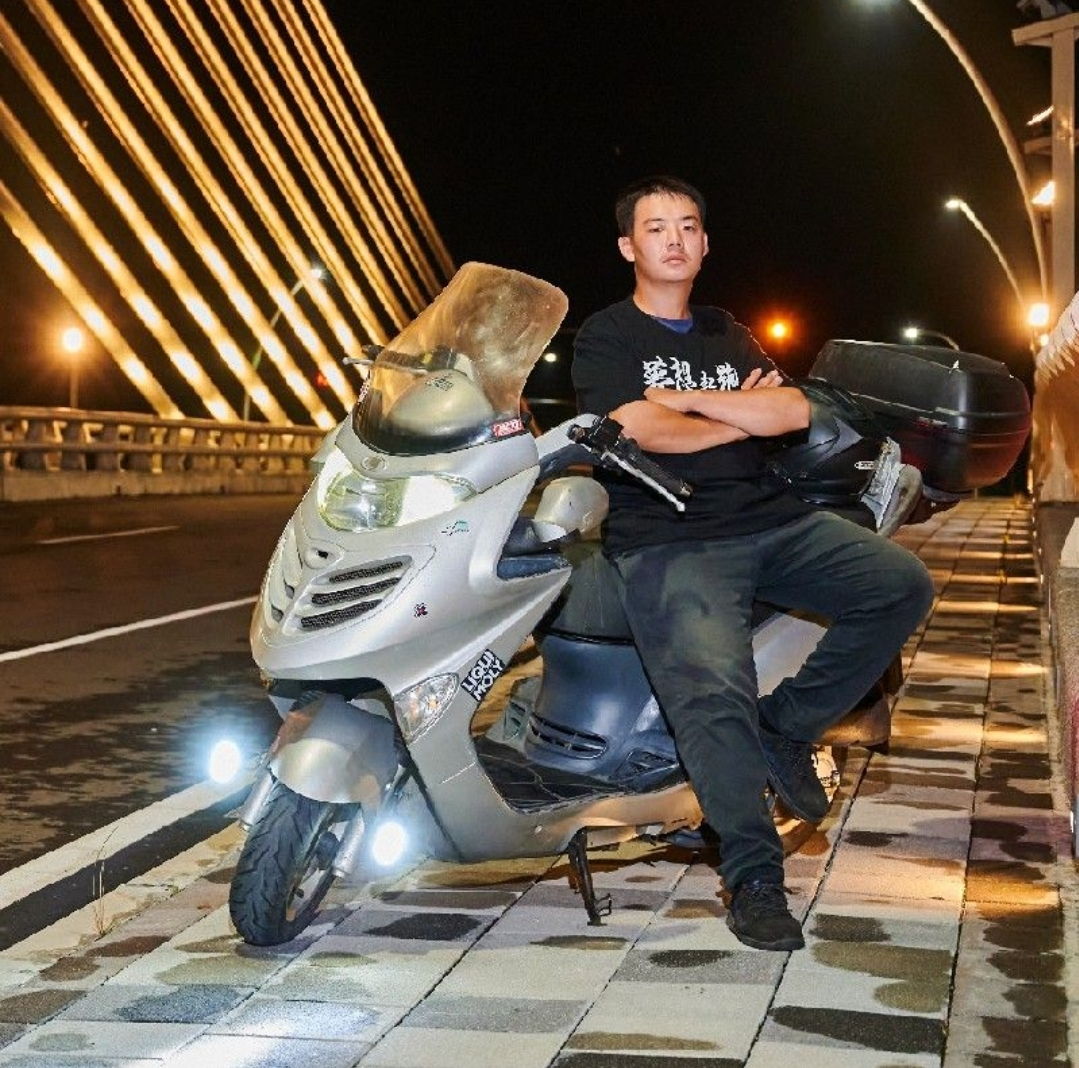
\includegraphics[width=1.15in]{41023251} %{}內是圖片文件的相對路徑
    \end{figure}
    \end{textblock}}
    {\renewcommand\baselinestretch{0.99}\selectfont %設定以下行距
    {\begin{textblock}{15}(3.5,4.3) %{寬度}(以左上角為原點之右移量,下移量)
\noindent\fontsize{14pt}{0em}\selectfont \makebox[4em][s]{姓名}\enspace:\enspace%\noindent指定首行不進行縮排
\fontsize{14pt}{0em}\selectfont \makebox[4em][s]{第三位}\\ 
\hspace*{\fill} \\
\noindent\fontsize{14pt}{0em}\selectfont \makebox[4em][s]{學號}\enspace:\enspace
\noindent\fontsize{14pt}{0em}\selectfont \makebox[4em][s]{41023251} \\ %\makebox為文本盒子
\hspace*{\fill} \\
\noindent\fontsize{14pt}{0em}\selectfont \makebox[4em][s]{就讀學校}\enspace:\enspace
\noindent\fontsize{14pt}{0em}\selectfont \makebox[9em][s]{國立虎尾科技大學}\\
\noindent\fontsize{14pt}{0em}\selectfont \makebox[5em][s]{\quad}\enspace\enspace
\noindent\fontsize{14pt}{0em}\selectfont \makebox[8em][s]{機械設計工程系}\\
\hspace*{\fill} \\
\noindent\fontsize{14pt}{0em}\selectfont \makebox[4em][s]{經歷}\enspace:\enspace
    \end{textblock}}}
   % \hspace*{\fill} \\
   \vspace{2em}
    {\begin{textblock}{6}(0,5.9)
    \begin{figure}
        
\includegraphics[width=1.15in]{41023254} %{}內是圖片文件的相對路徑
    \end{figure}
    \end{textblock}}
    {\renewcommand\baselinestretch{0.99}\selectfont %設定以下行距
    {\begin{textblock}{15}(3.5,6.1) %{寬度}(以左上角為原點之右移量,下移量)
\noindent\noindent\fontsize{14pt}{0em}\selectfont \makebox[4em][s]{姓名}\enspace:\enspace
\noindent\fontsize{14pt}{0em}\selectfont \makebox[4em][s]{第四位}\\ \hspace*{\fill} \\
\noindent\fontsize{14pt}{0em}\selectfont \makebox[4em][s]{學號}\enspace:\enspace
\noindent\fontsize{14pt}{0em}\selectfont \makebox[4em][s]{41023254} \\ \hspace*{\fill} \\
\noindent\fontsize{14pt}{0em}\selectfont \makebox[4em][s]{就讀學校}\enspace:\enspace
\noindent\fontsize{14pt}{0em}\selectfont \makebox[9em][s]{國立虎尾科技大學}\\
\noindent\fontsize{14pt}{0em}\selectfont \makebox[5em][s]{\quad}\enspace\enspace
\noindent\fontsize{14pt}{0em}\selectfont \makebox[8em][s]{機械設計工程系}\\
\hspace*{\fill} \\
\noindent\fontsize{14pt}{0em}\selectfont \makebox[4em][s]{經歷}\enspace:\enspace
    \end{textblock}}}
    %\hspace*{\fill} \\

\newpage
%=----------------書背----------------------=%
\pagestyle{empty}%設定沒有頁眉和頁腳
\begin{center}
\fontsize{0.001pt}{1pt}\selectfont .\\
\vspace{4em}
\fontsize{30pt}{30pt}\selectfont 【13】 \\
\fontsize{20pt}{20pt}\selectfont
\vspace{0.5em}
分\\
類\\
編\\
號\\
\vspace{0.5em}
\hspace{-0.5em}:\\
\vspace{0.5em}
\rotatebox[origin=cc]{270}{\sectionef\LARGE \textbf{pj3bg4}}\\ %旋轉
\vspace{0.5em}
網\\
際\\
足\\
球\\
場\\
景\\
設\\
計\\
\vspace{2em}
一\\
一\\
二\\
級\\

\end{center}
%\newpage
%\begin{landscape}  %橫式環境
%\begin{center}
%\fontsize{0.001pt}{1pt}\selectfont .
%\vspace{70mm}
%\rotatebox[origin=cc]{90}{\LARGE 【14】}\rotatebox[origin=cc]%{180}{\LARGE 1-2-APP-8765} %旋轉
%\end{center}
%\end{landscape}
\end{document}
